\section{Experiments}
\label{sec:experiments}
% 10-17 user request: figures for readers and abilities, fewer inline numbers; per-ability table moved to the appendix.

We compare \method{} with the systems of \cref{tab:systems} under the protocol of \cref{sec:setting}: tuned answer
prompt on BEAM, minimal prompt on LongMemEval, gpt-6-luna as judge, development sets only.

% E1: main results
\subsection{Main results}
\label{sec:main}
\begin{table}[t]
\centering\small
\caption{BEAM development sets, tuned answer prompt, gpt-6-luna judge. Mean of three runs except where
marked. Brackets: \method{} minus Hindsight\,+\,CC, 95\%
interval resampled by conversation, computed from unrounded scores. 200 questions (10 conversations) on BEAM-100K,
100 (5) on BEAM-1M. The tuned prompt is Mem0's public BEAM prompt, not tuned for any system here. $^\ddagger$one run.}
\label{tab:main}
\begin{tabular}{llrr}
\toprule
Reader & System & BEAM-100K & BEAM-1M \\
\midrule
\multirow{6}{*}{gpt-6-luna}
& Full context & \prelim{65.9}$^\ddagger$ & --- \\
& Record retrieval\,+\,CC & \prelim{69.7}$^\ddagger$ & \prelim{68.7}$^\ddagger$ \\
& Hindsight & \prelim{68.2} & \prelim{70.4} \\
& Hindsight\,+\,CC & \prelim{69.5} & \prelim{71.2} \\
& \method{} & \textbf{\prelim{76.8}} & \textbf{\prelim{75.4}} \\
& \quad $\Delta$ vs.\ Hindsight\,+\,CC & \prelim{$+7.3$ $[+4.5, +10.3]$} & \prelim{$+4.2$ $[+1.4, +8.3]$} \\
\midrule
\multirow{4}{*}{DeepSeek-V4.1-Flash}
& Hindsight & \prelim{75.3} & \prelim{75.2} \\
& Hindsight\,+\,CC & \prelim{76.0} & \prelim{76.7} \\
& \method{} & \textbf{\prelim{76.8}} & \textbf{\prelim{79.9}} \\
& \quad $\Delta$ vs.\ Hindsight\,+\,CC & \prelim{$+0.8$ $[-1.1, +2.9]$} & \prelim{$+3.2$ $[-0.6, +5.7]$} \\
\midrule
\multirow{4}{*}{gpt-6.1-sol}
& Hindsight & \prelim{76.8} & \prelim{78.8} \\
& Hindsight\,+\,CC & \prelim{77.0} & \prelim{78.9} \\
& \method{} & \textbf{\prelim{78.9}} & \textbf{\prelim{80.2}} \\
& \quad $\Delta$ vs.\ Hindsight\,+\,CC & \prelim{$+1.9$ $[-0.2, +3.9]$} & \prelim{$+1.3$ $[-3.0, +5.5]$} \\
\midrule
\multirow{4}{*}{gpt-6-astra$^\ddagger$}
& Hindsight & \prelim{75.3} & \prelim{80.4} \\
& Hindsight\,+\,CC & \prelim{76.7} & \prelim{79.5} \\
& \method{} & \textbf{\prelim{79.7}} & \textbf{\prelim{80.9}} \\
& \quad $\Delta$ vs.\ Hindsight\,+\,CC & \prelim{$+2.9$ $[+0.1, +5.6]$} & \prelim{$+1.4$ $[-4.8, +7.0]$} \\
\bottomrule
\end{tabular}
\end{table}

\paragraph{\method{} has the highest score in every cell; the gain is resolved with gpt-6-luna.}
\Cref{tab:main} gives the main comparison. With gpt-6-luna as reader, \method{} leads Hindsight\,+\,CC by 7 points on
BEAM-100K and 4 on BEAM-1M over three runs, and both intervals exclude zero. It also leads the record-retrieval system
that shares its records by about 7 points on both tiers; that system retrieves 8K characters and makes no compilation
call, and \cref{tab:ablation} separates the two factors. With the three stronger readers,
\method{} again has the highest score in all six cells, by about 1 to 3 points over Hindsight\,+\,CC, resolved only for
gpt-6-astra on BEAM-100K (\cref{sec:reader}).

\begin{figure}[t]
\centering
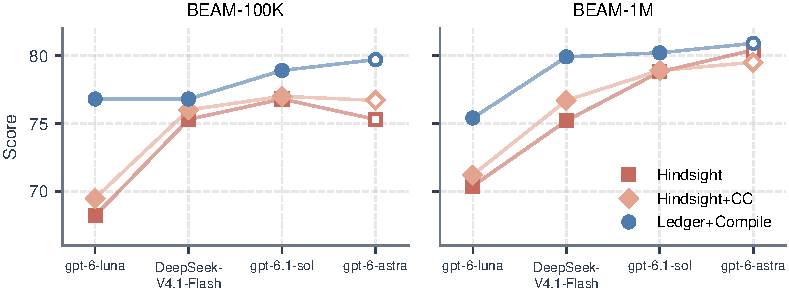
\includegraphics[width=0.98\linewidth]{figs/fig5_readers.pdf}
\caption{\textbf{Stronger readers close the gap.} Scores with four readers and the same memories (tuned prompt,
gpt-6-luna judge). Filled markers: mean of three runs; open markers: one run (gpt-6-astra, because of its
cost). Hindsight gains 6 to 10 points when gpt-6-luna is replaced by a stronger reader; \method{} gains
less, and stays ahead in every cell.}
\label{fig:readers}
\end{figure}

\paragraph{Gains concentrate on updates, instructions, and abstention; summarization is worse.}
\Cref{fig:ability} breaks the gpt-6-luna results down by ability (full table in \cref{app:detail}). Each ability has
only 20 questions on BEAM-100K and 10 on BEAM-1M, so single bars are noisy, but the pattern is consistent across the two
tiers. The largest gains are on knowledge update and instruction following on both tiers and on abstention on BEAM-100K,
followed by temporal reasoning and contradiction resolution, the abilities that the parts of the notes target
(\cref{sec:method}). \method{} is worse on summarization on both tiers, and roughly level on information extraction,
multi-session reasoning, and preference following. Summaries need broad coverage of a topic, which a 6,000-character
note that keeps exact items does not give; raising the limit to 15,000 characters did not help, because the notes
rarely used the extra room (\cref{app:detail}).

\begin{figure}[t]
\centering
\begin{minipage}[t]{0.48\linewidth}\vspace{0pt}\centering
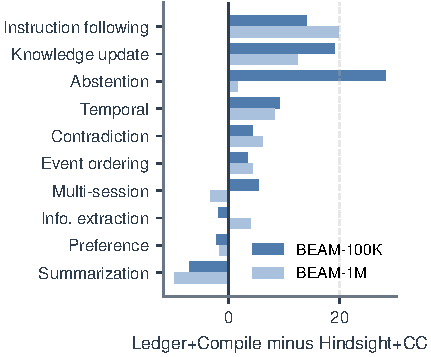
\includegraphics[width=\linewidth]{figs/fig6_ability.pdf}
\end{minipage}\hfill
\begin{minipage}[t]{0.48\linewidth}\vspace{4pt}
\caption{\textbf{Where \method{} gains and loses} (gpt-6-luna, three runs, difference to Hindsight\,+\,CC in points).
Knowledge update, instruction following, and abstention gain the most; summarization loses on both tiers. Each bar
covers 20 (BEAM-100K) or 10 (BEAM-1M) questions.}
\label{fig:ability}
\end{minipage}
\end{figure}

\paragraph{LongMemEval-S.}
We repeat the comparison on the 62 LongMemEval-S development questions with the minimal prompt, the same three
readers, and a Hindsight store built for each question's history (\cref{tab:lme}). \method{} is never below either
baseline. Its lead over Hindsight is largest with gpt-6-luna and smallest with gpt-6.1-sol, the same ordering as on
BEAM. One failure of Hindsight does not depend on the reader: on questions about what the assistant said earlier, it
answers about half correctly with every reader, while both record-based systems answer all of them, because its
extraction keeps mainly facts about the user. Most other questions are answered correctly by every system, so the
remaining differences are within the noise of 62 questions. \todo{test set.}

\begin{table}[t]
\centering
\small
\caption{LongMemEval-S development set (62 questions, minimal prompt, mean of three runs, gpt-6-luna judge).
Differences are \method{} minus the baseline, with 95\% paired bootstrap intervals over questions.}
\label{tab:lme}
\setlength{\tabcolsep}{4pt}
\resizebox{\linewidth}{!}{%
\begin{tabular}{lccccc}
\toprule
Reader & \method{} & Records (8K) & Hindsight & vs.\ records & vs.\ Hindsight \\
\midrule
gpt-6-luna & \prelim{84.4} & \prelim{82.3} & \prelim{71.0} & \prelim{$+2.2$} {\scriptsize[$-5.4$, $+10.8$]} & \prelim{$+13.4$} {\scriptsize[$+3.8$, $+23.1$]} \\
DeepSeek-V4.1-Flash & \prelim{93.5} & \prelim{86.6} & \prelim{85.5} & \prelim{$+7.0$} {\scriptsize[$+1.1$, $+13.4$]} & \prelim{$+8.1$} {\scriptsize[$+0.5$, $+16.1$]} \\
gpt-6.1-sol & \prelim{89.8} & \prelim{89.8} & \prelim{86.0} & \prelim{$+0.0$} {\scriptsize[$-4.8$, $+4.8$]} & \prelim{$+3.8$} {\scriptsize[$-6.5$, $+14.5$]} \\
\bottomrule
\end{tabular}}
\end{table}

% E2: reader strength
\subsection{What a stronger reader changes}
\label{sec:reader}
Changing the reader while keeping every memory fixed separates what the memory stores from how well the reader uses
it (\cref{fig:readers}). With the same 124K-character context, Hindsight\,+\,CC gains 6 to 10 points when gpt-6-luna
is replaced by DeepSeek-V4.1-Flash, gpt-6.1-sol, or gpt-6-astra, while \method{} gains at most about 5. \method{} stays
ahead in all eight reader-and-tier cells, but with the three stronger readers its lead over Hindsight\,+\,CC is 1 to 3
points and resolved only once (gpt-6-astra on BEAM-100K, one run). The stronger readers recover much of what Hindsight's long context
already contains, which is the reader loss of \cref{fig:loss}; compilation does that work in advance for a weaker
reader. On questions that need many facts at once, the strongest readers already do slightly better with Hindsight's
full context than with \method{}. The two are partly redundant, so \method{} helps most where the reader is weakest.
Intervals for every reader are in \cref{app:detail}.

% E3: ablations
\subsection{Ablations}
\label{sec:ablation}
\begin{table}[t]
\centering\small
\caption{Ablations with gpt-6-luna, tuned prompt, on questions about a single fact or state (point questions: 63 on
BEAM-1M, 128 on BEAM-100K). One run unless marked $^\star$ (three runs). The rows above the line use notes followed by
8K characters of records, the variant on which the components were developed.}
\label{tab:ablation}
\begin{tabular}{lrr}
\toprule
Variant & BEAM-100K & BEAM-1M \\
\midrule
Records only, 8K, + conflict check$^\star$ & \prelim{74.5} & \prelim{76.3} \\
Records only, 60K & --- & \prelim{74.3} \\
Notes from 60K + records 8K (full)$^\star$ & \prelim{81.6} & \prelim{80.7} \\
\quad without standing instructions$^\star$ & \prelim{77.9} & \prelim{79.1} \\
\quad notes only (reader sees $\approx$2K characters) & \prelim{79.6} & \prelim{78.2} \\
\quad notes compiled from 8K instead of 60K & \prelim{76.4} & \prelim{79.4} \\
\quad notes compiled from Hindsight's context$^\star$ & \prelim{75.0} & \prelim{77.6} \\
\midrule
Notes from 60K + records 60K (\method{})$^\star$ & \prelim{81.0} & \prelim{82.5} \\
\bottomrule
\end{tabular}
\end{table}

\paragraph{Compiling, not retrieving more, is the main effect.}
\Cref{tab:ablation} removes one component at a time on point questions. With the same 60K characters of records, the
reader scores about 6 points higher on BEAM-1M when it reads notes compiled from them than when it reads them directly,
so the gain does not come from retrieving more. Retrieving deeply before compiling matters more on BEAM-100K (about 6
points over compiling from 8K) than on BEAM-1M (about 1). Keeping records next to the notes adds 2 to 3 points, and the
standing-instruction part adds about 4 points on BEAM-100K over three runs, almost all of it on instruction following.

\paragraph{Each part of the notes helps the questions it targets.}
\Cref{tab:noteparts} removes one part of the notes at a time from the full method, on all 300 development questions
of both tiers. With gpt-6-luna, removing any part except ``not found'' lowers the score, but by only 1 to 2 points
overall, and only the standing instructions are resolved on their own. The effect of each part is concentrated on the
abilities it was written for: without standing instructions, instruction following drops by about 7 points; without
changes, knowledge update drops by about 6; and abstention drops whichever part is removed, because the structure
helps the reader decide whether the memory covers the question at all. The ``not found'' part has no measurable effect
and could be dropped. With gpt-6.1-sol no part has a resolved effect, and removing the standing instructions, if anything, helps
(one run on BEAM-100K: $+2.6$): a strong reader finds and follows earlier instructions in the records itself, while a weaker reader needs
them extracted. Single-run effects were about twice as large as three-run effects for gpt-6-luna, so we report three
runs where we have them.

\begin{table}[t]
\centering\small
\caption{Removing one part of the notes from \method{} (all 300 development questions of BEAM-100K and BEAM-1M,
tuned prompt, gpt-6-luna judge). Differences to the full notes, with 95\% intervals from a bootstrap over
conversations. gpt-6-luna: three runs; gpt-6.1-sol: two runs.}
\label{tab:noteparts}
\begin{tabular}{lcc}
\toprule
Variant & gpt-6-luna & gpt-6.1-sol \\
\midrule
Full notes (score) & \prelim{76.3} & \prelim{78.4} \\
\quad without standing instructions & \prelim{$-1.7$} {\scriptsize[$-3.1$, $-0.4$]} & \prelim{$+0.9$} {\scriptsize[$-0.3$, $+2.1$]} \\
\quad without changes & \prelim{$-1.3$} {\scriptsize[$-2.7$, $+0.2$]} & \prelim{$-0.0$} {\scriptsize[$-1.7$, $+1.6$]} \\
\quad without conflicts & \prelim{$-0.5$} {\scriptsize[$-1.7$, $+0.6$]} & \prelim{$+1.0$} {\scriptsize[$-0.3$, $+2.1$]} \\
\quad without not-found & \prelim{$+0.6$} {\scriptsize[$-1.2$, $+2.3$]} & \prelim{$-0.2$} {\scriptsize[$-1.9$, $+1.7$]} \\
\quad evidence only & \prelim{$-1.7$} {\scriptsize[$-3.5$, $+0.0$]} & \prelim{$+0.1$} {\scriptsize[$-1.8$, $+1.8$]} \\
\bottomrule
\end{tabular}
\end{table}
\todo{one run with DeepSeek-V4.1-Flash (running).}

\paragraph{Compiling from atomic records beats compiling from Hindsight's context.}
The same notes compiled from Hindsight's context instead of from atomic records lose about 7 points on BEAM-100K point
questions (resolved over three runs) and 3 on BEAM-1M (not resolved). The two sources also differ in length, 60K
characters of records against Hindsight's full 124K, so this compares two complete memories rather than two formats at
equal length. Notes still help Hindsight, by about 7 and 4 points over its own context, so compilation also works as a
plug-in. The gap is largest on abstention and knowledge update, where notes compiled from dated, self-contained records
can state when something changed and what was never said. Read directly, the two formats were close at equal budgets
(\cref{fig:budget}); the format starts to matter once something organizes it for the reader.

\paragraph{One input for all questions.}
Before arriving at \method{}, we routed questions about a whole topic to 60K characters of records and gave other
questions notes with 8K characters of records. Giving every question the notes with all 60K characters matches the
routed system over three runs on both tiers and removes the router; with DeepSeek-V4.1-Flash it is about 2 points
ahead on both tiers in one run.

\paragraph{On BEAM-1M, compiled notes are less sensitive to the answer prompt.}
On BEAM-1M point questions, switching from the minimal to the tuned prompt changes compiled notes by less than 1 point,
against about 5 for record retrieval with a conflict check and about 12 for Hindsight (one run each, on the
notes-plus-8K variant); on BEAM-100K all three change by at most about 2 points. On LongMemEval-S, where the tuned prompt was
not written for the benchmark, it lowers record retrieval by about 5 points, and notes with the minimal prompt score
highest. Compilation appears to do part of what the tuned prompt asks the reader to do, scanning everything and
cross-checking. \todo{repeat with \method{} and three runs.}

% E4: cost
\subsection{Cost}
\label{sec:cost}
\Cref{tab:cost} lists read-time tokens per question on BEAM-1M with gpt-6-luna. \method{} reads about 27K input tokens
over three calls, fewer than Hindsight's single answer call over its 124K-character context (33K) and fewer than
Hindsight\,+\,CC (47K); it writes more output tokens (1.5K against 0.4K and 0.2K), mostly the notes. The three calls
are sequential, so latency is roughly that of three model calls. At write time, \method{} makes one call per segment of
about 2K input and 1K output tokens. \todo{segments per conversation; Hindsight's write-time tokens.}

\begin{table}[t]
\centering\small
\caption{Average tokens per question at read time on BEAM-1M (gpt-6-luna; input / output, output includes reasoning; totals from unrounded values).}
\label{tab:cost}
\begin{tabular}{lrrrr}
\toprule
System & Plan & Conflict check / compile & Answer & Total \\
\midrule
Hindsight & --- & --- & \prelim{33.2K / 0.4K} & \prelim{33.2K / 0.4K} \\
Hindsight\,+\,CC & --- & \prelim{13.4K / 0.1K} & \prelim{33.7K / 0.2K} & \prelim{47.1K / 0.2K} \\
\method{} & \prelim{0.1K / 0.1K} & \prelim{12.4K / 1.0K} & \prelim{14.7K / 0.4K} & \prelim{27.2K / 1.5K} \\
\bottomrule
\end{tabular}
\end{table}

% E5: test sets
\subsection{Held-out test sets}
\label{sec:test}
We ran the test sets once, after freezing \method{}, its prompts and the baselines' configurations: the 10
BEAM-100K conversations not used for development (200 questions), BEAM-1M conversations 6--15 (200 questions), and
the 151 LongMemEval-S test questions. Readers, judge, prompts and intervals are those of \cref{tab:main}; on
LongMemEval-S the interval is resampled by question.

\begin{table}[t]
\centering\small
\caption{Held-out test sets, gpt-6-luna reader and judge, mean of three runs. Brackets: \method{} minus the
system in that row, 95\% interval (BEAM: resampled by conversation; LongMemEval-S: by question). Point / aggregate:
questions routed to each answer path (\cref{sec:method}); Hindsight\,+\,CC equals Hindsight on aggregate questions.}
\label{tab:test}
\begin{tabular}{lrrr}
\toprule
System & BEAM-100K & BEAM-1M & LongMemEval-S \\
\midrule
LycheeMemory & --- & --- & \prelim{83.2} \\
Hindsight & \prelim{64.9} & \prelim{61.5} & \prelim{78.6} \\
Hindsight\,+\,CC & \prelim{67.6} & \prelim{64.4} & --- \\
\method{} & \textbf{\prelim{73.7}} & \textbf{\prelim{71.2}} & \textbf{\prelim{85.0}} \\
\midrule
$\Delta$ vs.\ Hindsight & \prelim{$+8.8$ $[+3.7, +13.9]$} & \prelim{$+9.6$ $[+6.4, +12.8]$} & \prelim{$+6.4$ $[+0.9, +11.9]$} \\
$\Delta$ vs.\ Hindsight\,+\,CC & \prelim{$+6.1$ $[+1.1, +10.7]$} & \prelim{$+6.8$ $[+3.4, +10.2]$} & --- \\
$\Delta$ vs.\ LycheeMemory & --- & --- & \prelim{$+1.8$ $[-2.4, +6.0]$} \\
\midrule
Point questions (ours / H+CC / H) & \prelim{76.8 / 67.6 / 63.4} & \prelim{70.2 / 56.8 / 52.0} & --- \\
Aggregate questions (ours / H) & \prelim{67.9 / 67.6} & \prelim{72.6 / 75.3} & --- \\
\bottomrule
\end{tabular}
\end{table}

\paragraph{The development-set gains hold on the test sets.}
\Cref{tab:test} repeats the main comparison on data not used for any decision. On both BEAM tiers \method{} leads
Hindsight\,+\,CC by 6 to 7 points with intervals that exclude zero, as on the development sets (7.3 and 4.2). The
lead comes from questions routed to the point path, where it is 9 to 13 points; on aggregate questions \method{} ties
Hindsight on BEAM-100K and trails it by 2.7 points on BEAM-1M, matching its weakness on summarization
(\cref{sec:limits}). On LongMemEval-S \method{} leads Hindsight by 6.4 points (interval excludes zero) and
LycheeMemory by 1.8 (it does not), the same pattern as on the development set. Every system scores lower on the test
conversations than on the development ones (by 2 to 9 points), most of all Hindsight on BEAM-1M, so the gain does not
shrink on harder data. While building records for LongMemEval-S, the provider's content filter blocked the encoding
output for two segments; those segments contribute no records, and all questions are kept.
\todo{Stronger reader (gpt-6.1-sol) on the test sets.}
